\documentclass[12pt]{article}
\usepackage{../../../lecture_notes}
\usepackage{../../../math}
\usepackage{../../../uark_colors}

\hypersetup{
  colorlinks = true,
  allcolors = ozark_mountains,
  breaklinks = true,
  bookmarksopen = true
}

\begin{document}
\begin{center}
  {\Huge\bf Midterm 1 - Fall 2024}
  
  \smallskip
  {\large\it  ECON 4753 — University of Arkansas}
\end{center}

\vspace{5mm}
\begin{enumerate}
  \item Say you have a sample of 100 companies where you observe the average wage and the number of non-managerial employees. You regress the $\log$ of average wage at a company on the number of non-managerial employees and estimate a coefficient of $\hat{\beta}_1 = 0.005$. Interpret this coefficient estimate in words.
  




  \vspace{5mm}
  \item Below is a graph using data from law schools. Along the X axis is the rank of the law school (1 is best) and along the Y axis is the median starting salary for graduates. On the chart, I have ploted estimates from a linear regression of $Y$ on $X$ and a fourth-order polynomial of $X$.
  \begin{enumerate}
    \item How would I evaluate which model performs `better' on this sample?
    
    \item Describe which of the two models you would use if your goal is predicting median starting salary given the rank of a law school? 
    
    \item Why might someone want to use the linear model in this context?
  \end{enumerate}

  \begin{center}
    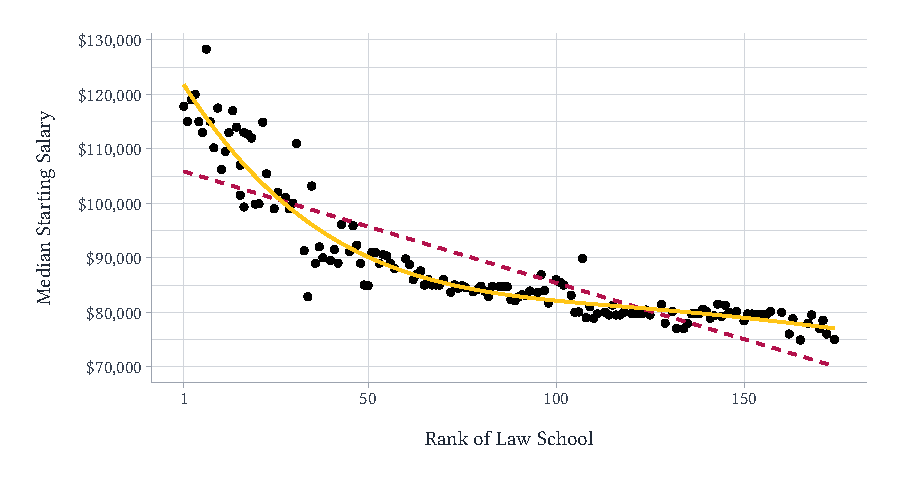
\includegraphics[width = 0.85\textwidth]{figures/plot_law_school_rank_and_salary.pdf}
  \end{center}





  \vspace{5mm}
  \item Continuing with the law school example, say we regress salary on an intercept and an indicator being a top 25 ranked program (=1 if ranked in top 25, =0 otherwise). We estimate a coefficient of 27177 and a standard error of 1528. 
  \begin{enumerate}
    \item Can you reject the null that top 25 ranked law schools do not earn more than other law schools?
  \end{enumerate}




  \vspace{5mm}
  \item Continuing with the law school example, the regression model estimate is as follows: 
  \begin{codeblock}[{}]
OLS estimation, Dep. Var.: salary
               Estimate  Std. Error   t value   Pr(>|t|)    
(Intercept)  106063.518   1405.0819   75.4856  < 2.2e-16 ***
rank           -206.731     12.5843  -16.4278  < 2.2e-16 ***
---
Signif. codes:  0 '***' 0.001 '**' 0.01 '*' 0.05 '.' 0.1 ' ' 1
  \end{codeblock}

  \begin{enumerate}
    \item Interpret the coefficient on a law school's \texttt{rank}
    
    \item Form a 95\% confidence interval for the rank coefficient (the critical value of the middle 95\% is $\pm 1.96$).
  \end{enumerate}
  



  \vspace{5mm}
  \item Continuing with the law school example, schools can be broken up into 4 US regions: Northeast, South, Midwest, and the West. We want to see if different regions have different starting salaries. We regress median starting salaries on dummies for each region (excluding one)
  \begin{codeblock}[{}]
OLS estimation, Dep. Var.: salary
                    Estimate Std. Error   t value  Pr(>|t|)    
(Intercept)        88366.52    2143.09 41.233212 < 2.2e-16 ***
region::Northeast   3874.39    3097.83  1.250681   0.21308    
region::South      -4025.82    2499.87 -1.610412   0.10950    
region::West        1568.09    2828.93  0.554307   0.58023    
---
Signif. codes:  0 '***' 0.001 '**' 0.01 '*' 0.05 '.' 0.1 ' ' 1
  \end{codeblock}

  \begin{enumerate}
    \item What is the omitted group in this case?

    \item What is the average median starting salary for lawyers who went to school in the West? 
  \end{enumerate}

\end{enumerate}



\end{document}
